% steps/step03.tex
\section[گام سوم: جمع‌آوری داده]{\faDatabase\ \ گام سوم: جمع‌آوری داده}
\begin{stepbox}

\field{چه نوع داده‌هایی لازم است؟}{
    داده‌های مورد نیاز این پروژه شامل دو بخش اصلی است: نخست، داده خام یعنی اسکن‌های سه‌بعدی توموگرافی کامپیوتری (\lr{CT Scan}) از ناحیه شکم که ترجیحاً در فاز وریدی (\lr{Portal Venous Phase}) ثبت شده‌اند؛ زیرا در این فاز، اختلاف کنتراست میان بافت سالم کبد و ضایعات تومورال بیشینه می‌شود. این داده‌ها به‌صورت حجم‌های سه‌بعدی و در قالب فرمت \lr{NIfTI} (\texttt{.nii}) برای ورود به مدل پردازش می‌شوند. دوم، برچسب‌های مرجع (\lr{Ground Truth}) شامل ماسک‌های سه‌بعدی متناظر با هر اسکن است که توسط رادیولوژیست‌های متخصص به‌صورت دستی حاشیه‌نویسی شده‌اند. این ماسک‌ها معمولاً سه کلاس را شامل می‌شوند: پس‌زمینه (کد ۰)، بافت سالم کبد (کد ۱) و تومور (کد ۲).
}

\field{منابع داده کدام‌اند؟}{
    منبع اصلی و بهینه برای این مرحله، دیتاست‌های استاندارد و اعتبارسنجی‌شده جهانی مانند \lr{LiTS (Liver Tumor Segmentation Benchmark)} است که از طریق پلتفرم‌هایی نظیر \lr{Kaggle} نیز در دسترس قرار دارد. این داده‌ها از دستگاه‌ها و پروتکل‌های تصویربرداری بیمارستان‌های مختلف گردآوری شده‌اند و همین تنوع، نقش مهمی در کاهش بیش‌برازش (\lr{Overfitting}) و افزایش توان تعمیم‌پذیری مدل نهایی دارد.
}

\field{ملاحظات حریم خصوصی و قانونی چیست؟}{
    پردازش تصاویر پزشکی مستقیماً با قوانین سخت‌گیرانه حفاظت از داده‌های سلامت، مانند \lr{HIPAA} و \lr{GDPR}، در ارتباط است. مهم‌ترین الزام در این بخش، بی‌نام‌سازی کامل (\lr{Anonymization / De-identification}) داده‌ها است. فایل‌های پزشکی در قالب اصلی خود، یعنی \lr{DICOM}، شامل هدرهایی دارای اطلاعات هویتی حساس بیمار (\lr{PHI}) مانند نام، تاریخ تولد و کد ملی هستند. بنابراین، پاک‌سازی کامل این متادیتاها و تبدیل ایمن داده‌ها به فرمت \lr{NIfTI} پیش از ورود به فرآیند آموزش مدل، یک الزام قانونی و اخلاقی غیرقابل‌مذاکره محسوب می‌شود.
}

\begin{center}
    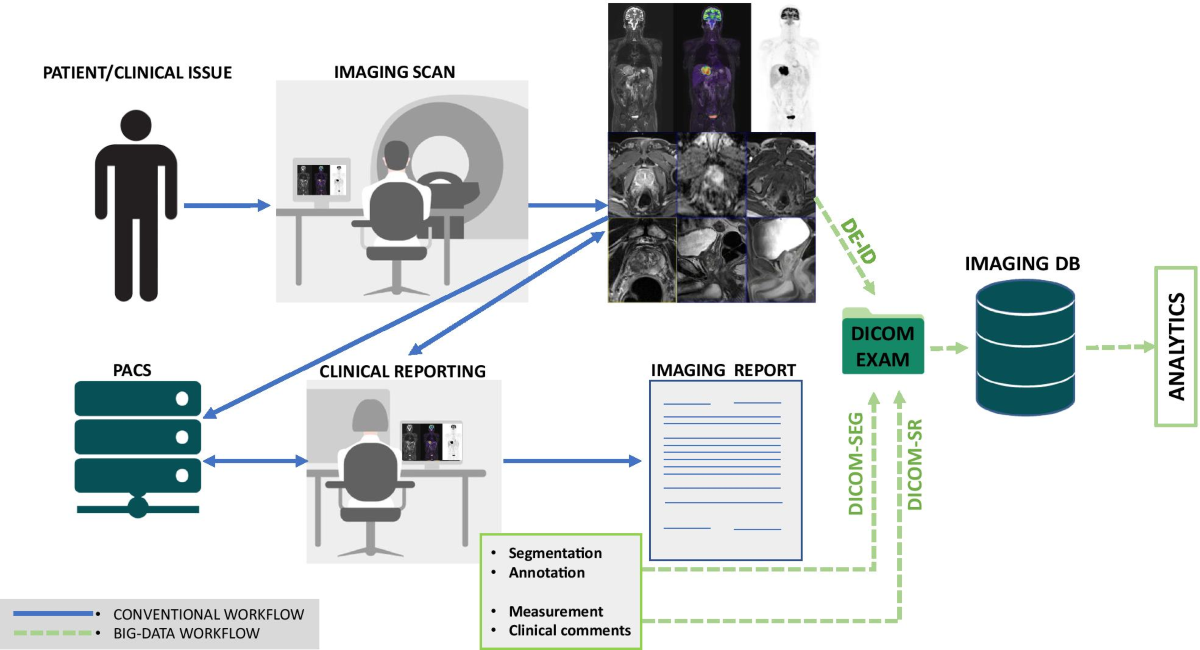
\includegraphics[width=0.85\textwidth]{images/dicom.png}
    \vspace{0.2cm} \\
    \footnotesize{شکل ۳ - مسیر گردش داده‌های تصویربرداری پزشکی از محیط بالینی به پایگاه‌داده‌های تحلیلی. فلش‌های نقطه‌چینِ سبزرنگ فرآیند بی‌نام‌سازی (\lr{DE-ID}) را پیش از ورود داده‌ها به سیستم‌های پردازشی نشان می‌دهند.}
\end{center}


\end{stepbox}
